\sectionnonum{Įvadas}

\subsection*{Praktikos vieta}
Pasirinkta praktikos vieta -- \SEB, \PDT. Pagrindinė šios praktikos vietos pasirinkimo priežastis -- tai yra dabartinė autoriaus darbo vieta, kurioje autorius susiduria su visais programų sistemų kūrimo etapais ir iššūkiais bei juos sprendžia. 

\subsection*{Problematika}
Vienoje iš banko sistemų naudojamas automatinis tam tikrų duomenų bazės įrašų versijavimas (t.~y. kaskart atliekant įrašo pakeitimą sukuriamas naujas įrašas kitoje duomenų bazės lentelėje išsaugantis tiek keitimo faktą, tiek keičiamo įrašo originalią versiją). Pastebėta, jog toks įrašų versijavimas sukuria didelį duomenų kiekį, kuris ilgainiui padidina duomenų bazės apkrovą. Pagrindinis praktikos uždavinys -- atlaisvinti vietą duomenų bazėje ir sumažinti jos apkrovą.

\subsection*{Praktikos tikslas ir uždaviniai}
Kadangi įrašų versijavimas yra nuolatinis procesas, vietos atlaisvinimas taip pat turi vykti nuolat ir negali sukurti nuolatinio papildomo darbo įmonės darbuotojams. Iš tokių reikalavimų kyla pagrindinis praktikos tikslas -- sukurti automatizuotą versijavimo įrašų archyvavimo sprendimą.

Kuriant šį sprendimą turi būti atsižvelgta į esamus procesus bei organizacijoje naudojamas ir patvirtinas technologijas. Šių reikalavimų kontekste formuojami praktikos uždaviniai tikslui pasiekti:
\begin{itemize}
    \item Išanalizuoti organizacijoje naudojamas duomenų saugyklas ir parinkti tinkamiausią,
    \item įgyvendinti integraciją tarp parinktos duomenų saugyklos ir programų sistemos,
    \item sukurti ir įgyvendinti automatinio duomenų archyvavimo procesą,
    \item sukurti ir įgyvendinti archyvuotų duomenų peržiūros ir palyginimo naudotojo sąsają.
\end{itemize}   

\subsection*{Praktinės veiklos planas ir atlikimo eiga}

Praktinės veiklos planas pateiktas \ref{fig:plan}-ame pav. Jame aprašytos numatytos praktikos veiklos bei nurodyti svarbiausi tarpiniai veiklos rezultatai (artefaktai ar priimti sprendimai, pavyzdžiui, \textit{Duomenų gyvavimo ciklo} artefaktas). Plane taip pat rodyklėmis nurodyta veiklų eiga. 

\begin{figure}
    \centering
    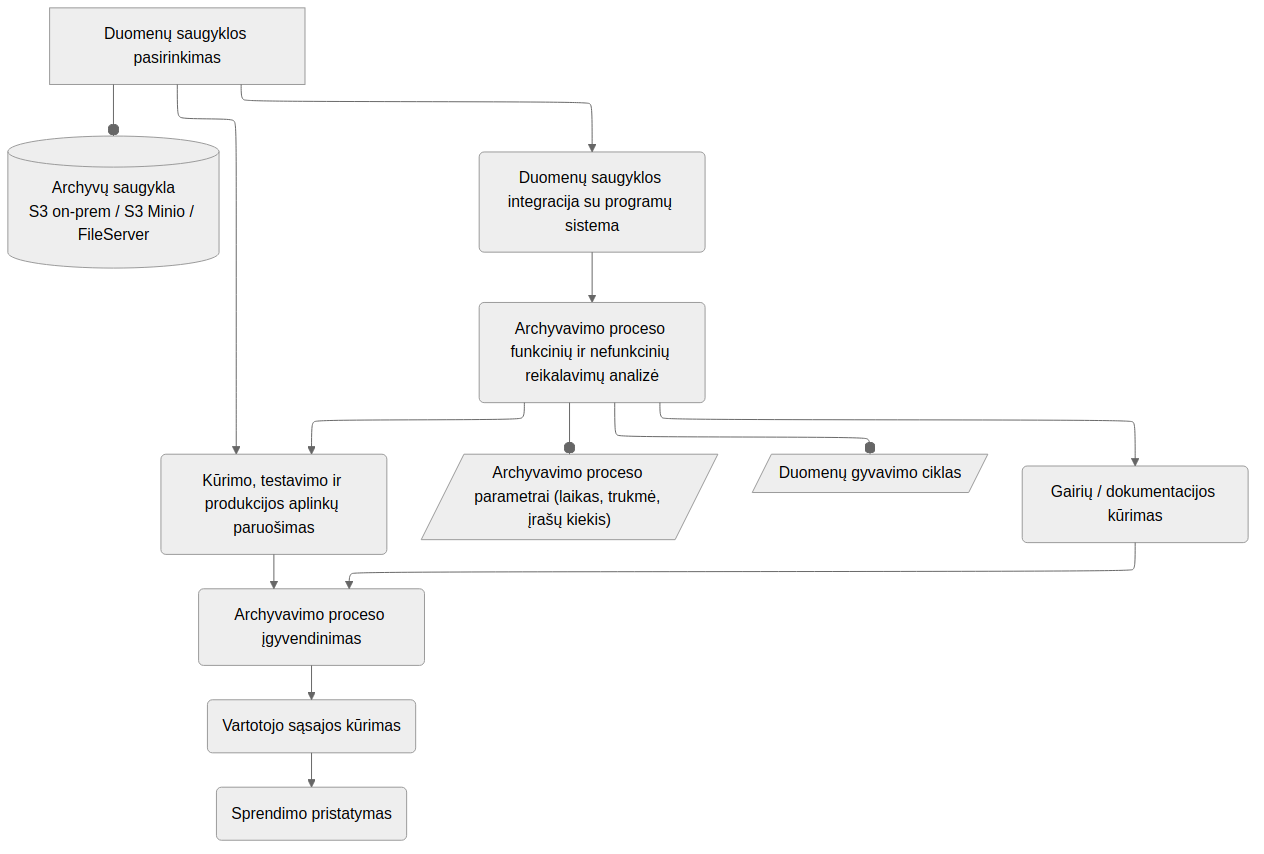
\includegraphics[width=\textwidth]{images/plan.png}
    \caption{Praktinės veiklos planas}
    \label{fig:plan}
\end{figure}
